\documentclass[report.tex]{subfiles}

\begin{document}

\section{Thiết kế cơ sở dữ liệu}

\subsection{Mô hình ERD}

\begin{figure}[!htb]
{\centering
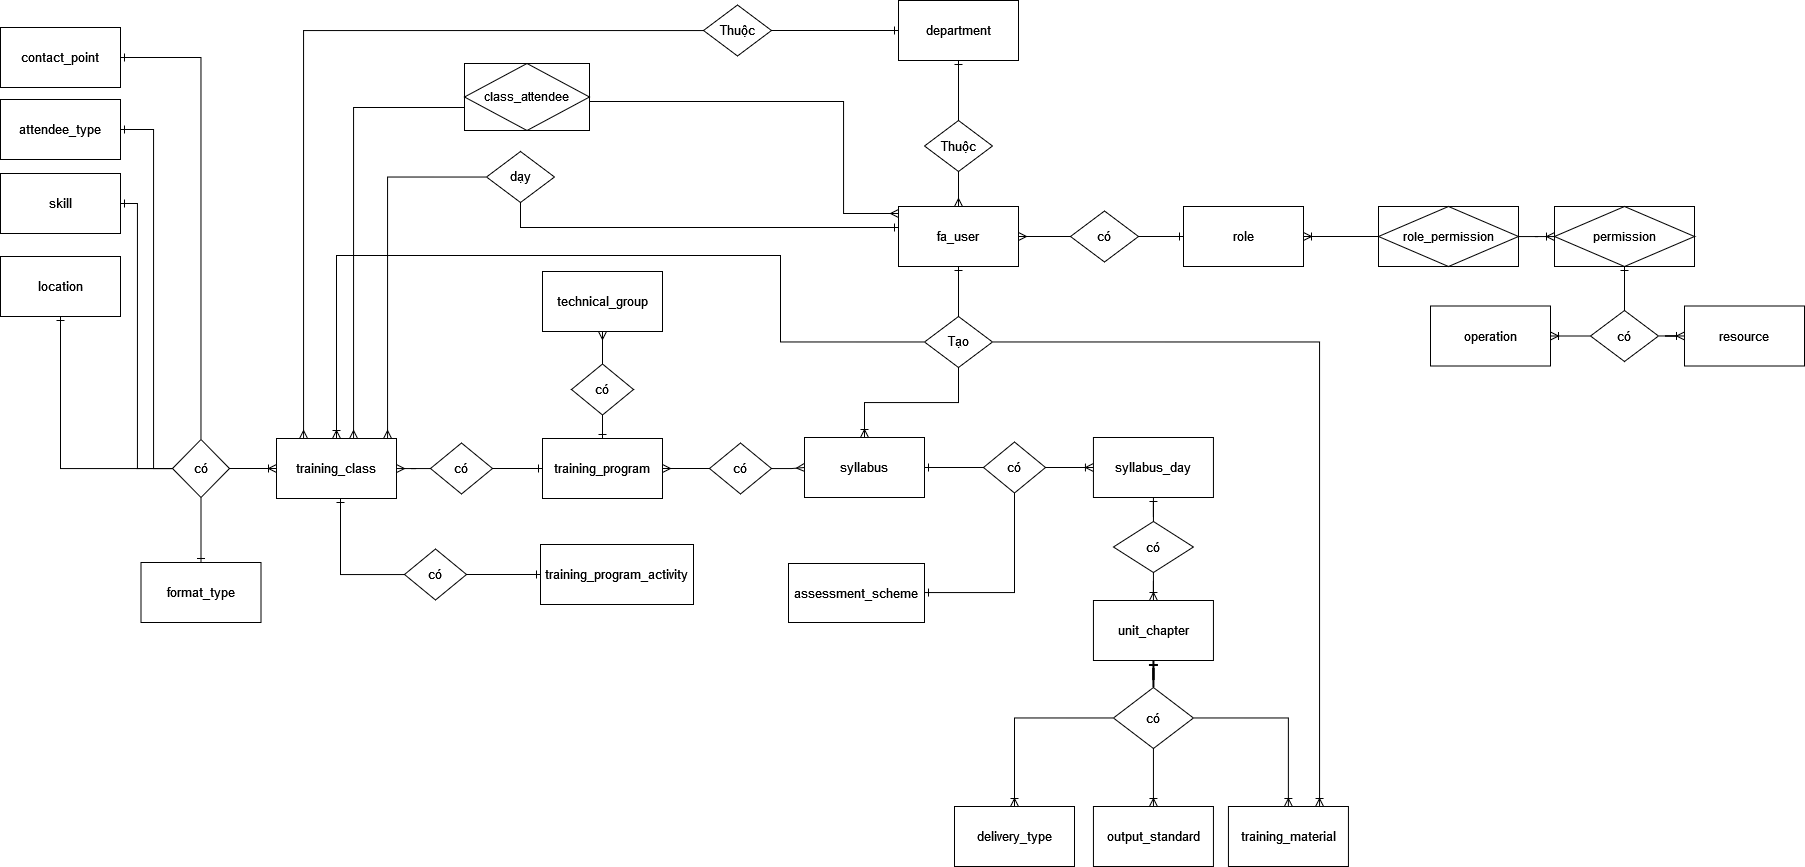
\includegraphics[width=500px]{../meta/db.erd.png}
\caption{Mô hình ERD}
\par
}
\end{figure}
\FloatBarrier

\subsection{Chuẩn hóa dữ liệu}

Quy ước:

- Primary key: (gạch chân) \underline{id} \\
- Foreign key: (in đậm) \textbf{other\_id} \\
- Composite key: (gạch chân, in đậm): \textbf{\underline{id\_1, id\_2}} \\

\begin{enumerate}[nosep]
\item[--] \textbf{fa\_user}: \underline{id}, created\_by, created\_time, updated\_by, updated\_time, uuid, address, avatar, birthdate, disabled, email, expired, full\_name, gender, locked, password, status, username, \textbf{department\_id}, \textbf{role\_id}
\item[--] \textbf{syllabus}: \underline{id}, created\_by, created\_date, is\_deleted, updated\_by, updated\_date, uuid, ancestor, attendee\_number, code, course\_objective, days, delivery\_principle, hours, level, name, status, technical\_requirement, version
\item[--] \textbf{syllabus\_day}: \underline{id}, created\_by, created\_date, is\_deleted, updated\_by, updated\_date, uuid, day\_no, syllabus\_id
\item[--] \textbf{syllabus\_unit}: \underline{id}, created\_by, created\_date, is\_deleted, updated\_by, updated\_date, uuid, duration, name, unit\_no, syllabus\_day\_id
\item[--] \textbf{unit\_chapter}: \underline{id}, created\_by, created\_date, is\_deleted, updated\_by, updated\_date, uuid, chapter\_no, duration, is\_online, name, delivery\_type\_id, output\_standard\_id, syllabus\_unit\_id
\item[--] \textbf{assessment\_scheme}: \underline{id}, assignment, final\_practice, final, final\_theory, gpa, quiz, \textbf{syllabus\_id}
\item[--] \textbf{training\_material}: \underline{id}, created\_by, created\_date, is\_deleted, updated\_by, updated\_date, uuid, file\_name, is\_file, name, url, unit\_chapter\_id
\item[--] \textbf{training\_program}: \underline{id}, created\_by, created\_date, updated\_by, updated\_date, uuid, code, days, hours, issued\_date, issued\_status, name, status, attendee\_id, position\_id, technical\_group\_id
\item[--] \textbf{training\_class}: \underline{id}, created\_by, created\_date, updated\_by, updated\_date, uuid, accepted\_attendee, actual\_attendee, actual\_end\_date, actual\_start\_date, class\_status, code, duration, end\_time, expected\_end\_date, expected\_start\_date, name, planned\_attendee, remark, slot\_time, start\_time, attendee\_level\_id, class\_training\_program\_id, format\_type\_id, department\_id, position\_id, skill\_id
\item[--] \textbf{class\_attendee}: \underline{id}, username, \textbf{training\_class\_id}, \textbf{\underline{username, training\_class\_id}}
\item[--] \textbf{training\_program\_activity}: \underline{id}, days, hours, sort, uuid, class\_training\_program\_id, created\_by, created\_date, description, name, updated\_by, updated\_date
\item[--] \textbf{technical\_group}: \underline{technical\_group\_id}, description, technical\_group\_name
\item[--] \textbf{contact\_point}: \underline{id}, content, type, department\_id
\item[--] \textbf{attendee\_type}: \underline{attendee\_type\_id}, description, attendee\_type\_name
\item[--] \textbf{delivery\_type}: \underline{id}, descriptions, icon, name
\item[--] \textbf{format\_type}: \underline{id}, abbreviation, name
\item[--] \textbf{department}: \underline{id}, name, description
\item[--] \textbf{output\_standard}: \underline{id}, code, descriptions, name
\item[--] \textbf{position}: \underline{position\_id}, description, position\_name
\item[--] \textbf{location}: \underline{id}, address, name, site
\item[--] \textbf{skill}: \underline{id}, name
\item[--] \textbf{resource}: \underline{id}, created\_by, created\_time, updated\_by, updated\_time, uuid, name
\item[--] \textbf{operation}: \underline{id}, created\_by, created\_time, updated\_by, updated\_time, uuid, name
\item[--] \textbf{role}: \underline{id}, created\_by, created\_time, updated\_by, updated\_time, uuid, name
\item[--] \textbf{role\_permission}: \underline{role\_id}, permission\_id
\item[--] \textbf{permission}: \underline{id}, created\_by, created\_time, updated\_by, updated\_time, uuid, name, operation\_id, resource\_id
\end{enumerate}

\subsection{Từ điển dữ liệu}

\begin{table}[!htb]
\begin{longtable}{|p{3cm}|p{3cm}|p{1cm}|p{1.6cm}|p{5cm}|}
\hline
\textbf{Tên cột} & \textbf{Kiểu dữ liệu} & \textbf{PK} & \textbf{Nullable} & \textbf{Mô tả} \\
\hline
created\_by & varchar & & X & username tạo \\
created\_date & timestamp & & X & Thời điểm tạo \\
updated\_by & varchar & & X & username cập nhật \\
updated\_date & timestamp & & X & Thời điểm cập nhật \\
is\_deleted & boolean & & X & đã xóa \\
uuid & uuid & & & UUID \\
code & varchar & & X & Mã \\
course\_objective & bytea & & X & Mô tả nội dung \\
delivery\_principle & bytea & & X & Văn bản \\
technical\_requirement & bytea & & X & Văn bản \\
days & integer & & X & Số ngày \\
hours & double & & X & Số giờ \\
name & varchar & & & Tên \\
status & varchar & & & Trạng thái \\
version & varchar & & & Phiên bản \\
id & bigint & X & & Identifier \\
\hline
\caption[Bảng syllabus]{Bảng syllabus: nội dung đào tạo}
\end{longtable}
\end{table}
\FloatBarrier

\begin{table}[!htb]
\begin{longtable}{|p{3cm}|p{3cm}|p{1cm}|p{1.6cm}|p{6cm}|}
\hline
\textbf{Tên cột} & \textbf{Kiểu dữ liệu} & \textbf{PK} & \textbf{Nullable} & \textbf{Mô tả} \\
\hline
created\_by & varchar & & Yes & username tạo \\
created\_date & timestamp & & Yes & Thời điểm tạo \\
is\_deleted & boolean & & & \\
updated\_by & varchar & & & username cập nhật \\
updated\_date & timestamp & & & Thời điểm cập nhật \\
uuid & uuid & & & UUID \\
day\_no & integer & & & \\
syllabus\_id & bigint & & & \\
id & bigint & X & & Identifier \\
\hline
\caption[Bảng syllabus\_day]{Bảng syllabus\_day: ngày trong NDDT}
\end{longtable}
\end{table}
\FloatBarrier

\pagebreak %

\begin{table}[!htb]
\begin{longtable}{|p{3cm}|p{3cm}|p{1cm}|p{1.6cm}|p{6cm}|}
\hline
\textbf{Tên cột} & \textbf{Kiểu dữ liệu} & \textbf{PK} & \textbf{Nullable} & \textbf{Mô tả} \\
\hline
created\_by & varchar & & Yes & username tạo \\
created\_date & timestamp & & Yes & Thời điểm tạo \\
is\_deleted & boolean & & & \\
updated\_by & varchar & & & username cập nhật \\
updated\_date & timestamp & & & Thời điểm cập nhật \\
uuid & uuid & & & UUID \\
chapter\_no & integer & & & \\
duration & integer & & & \\
is\_online & boolean & & & \\
name & varchar & & & \\
delivery\_type\_id & bigint & & & PTDT \\
output\_standard\_id & bigint & & & TCDR \\
syllabus\_unit\_id & bigint & & & Nội dung \\
id & bigint & X & & \\
\hline
\caption[Bảng chapter]{Bảng chapter: thông tin một chương trong NDDT}
\end{longtable}
\end{table}
\FloatBarrier

\begin{table}[!htb]
\begin{longtable}{|p{3cm}|p{3cm}|p{1cm}|p{1.6cm}|p{6cm}|}
\hline
\textbf{Tên cột} & \textbf{Kiểu dữ liệu} & \textbf{PK} & \textbf{Nullable} & \textbf{Mô tả} \\
\hline
created\_by & varchar & & Yes & username tạo \\
created\_date & timestamp & & Yes & Thời điểm tạo \\
updated\_by & varchar & & Yes & username cập nhật gần nhất \\
updated\_date & timestamp & & Yes & Thời điểm cập nhật gần nhất \\
uuid & uuid & & & UUID \\
code & varchar & & & Mã \\
days & integer & & & Số ngày \\
hours & integer & & & Số giờ \\
name & varchar & & & Tên \\
status & integer & & & trạng thái \\
attendee\_id & bigint & & & ID loại học viên \\
position\_id & bigint & & & ID vị trí \\
technical\_group\_id & bigint & & & ID mã kỹ thuật \\
id & bigint & X & & Identifier \\
\hline
\caption[Bảng training\_program]{Bảng training\_program: CTDT}
\end{longtable}
\end{table}
\FloatBarrier

\begin{table}[!htb]
\begin{longtable}{|p{3cm}|p{3cm}|p{1cm}|p{1.6cm}|p{6cm}|}
\hline
\textbf{Tên cột} & \textbf{Kiểu dữ liệu} & \textbf{PK} & \textbf{Nullable} & \textbf{Mô tả} \\
\hline
created\_by & varchar & & Yes & username tạo \\
created\_date & timestamp & & Yes & Thời điểm tạo \\
is\_deleted & boolean & & & Đã xóa \\
updated\_by & varchar & & & username cập nhật \\
updated\_date & timestamp & & & Thời điểm cập nhật \\
uuid & uuid & & & UUID \\
duration & integer & & & Thời gian \\
name & varchar & & & Tên \\
unit\_no & integer & & & STT unit \\
syllabus\_day\_id & bigint & & & ID ngày \\
id & bigint & X & & Identifier \\
\hline
\caption[Bảng syllabus\_unit]{Bảng syllabus\_unit}
\end{longtable}
\end{table}
\FloatBarrier

\begin{table}[!htb]
\begin{longtable}{|p{3cm}|p{3cm}|p{1cm}|p{1.6cm}|p{6cm}|}
\hline
\textbf{Tên cột} & \textbf{Kiểu dữ liệu} & \textbf{PK} & \textbf{Nullable} & \textbf{Mô tả} \\
\hline
assignment & double & & & \% điểm bài tập \\
gpa & double & & & GPA \\
quiz & double & & & \% điểm trả lời câu hỏi \\
syllabus\_id & bigint & & & ID NDDT \\
final & double & & & \% điểm kiểm tra \\
final\_practice & double & & & \% điểm thực hành \\
final\_theory & double & & & \% điểm lý thuyết \\
id & bigint & X & & Identifier \\
\hline
\caption[Bảng assessment\_scheme]{Bảng assessment\_scheme: quy cách tính điểm cho NDDT}
\end{longtable}
\end{table}
\FloatBarrier

\begin{table}[!htb]
\begin{longtable}{|p{3cm}|p{3cm}|p{1cm}|p{1.6cm}|p{6cm}|}
\hline
\textbf{Tên cột} & \textbf{Kiểu dữ liệu} & \textbf{PK} & \textbf{Nullable} & \textbf{Mô tả} \\
\hline
created\_by & varchar & & Yes & username tạo \\
created\_date & timestamp & & Yes & Thời điểm tạo \\
is\_deleted & boolean & & & Đã xóa \\
updated\_by & varchar & & & username cập nhật \\
updated\_date & timestamp & & & Thời điểm cập nhật \\
uuid & uuid & & & UUID \\
file\_name & varchar & & & tên file \\
is\_file & boolean & & & file \\
name & varchar & & & Tên \\
url & varchar & & & URL của NDDT \\
unit\_chapter\_id & bigint & & & Chapter ID \\
id & bigint & X & & Identifier \\
\hline
\caption[Bảng training\_material]{Bảng training\_material: TLDT}
\end{longtable}
\end{table}
\FloatBarrier


\begin{table}[!htb]
\begin{longtable}{|p{3cm}|p{3cm}|p{1cm}|p{1.6cm}|p{6cm}|}
\hline
\textbf{Tên cột} & \textbf{Kiểu dữ liệu} & \textbf{PK} & \textbf{Nullable} & \textbf{Mô tả} \\
\hline
created\_by & varchar & & Yes & username tạo \\
created\_date & timestamp & & Yes & Thời điểm tạo \\
updated\_by & varchar & & Yes & username cập nhật gần nhất \\
updated\_date & timestamp & & Yes & Thời điểm cập nhật gần nhất \\
uuid & uuid & & & UUID \\
actual\_attendee & integer & & & Số lượng học viên \\
expected\_end\_date & date & & & Ngày mở lớp \\
expected\_start\_date & date & & & Ngày lớp kết thúc \\
start\_time & time & & & Thời gian vào lớp \\
end\_time & time & & & Thời gian tan lớp \\
class\_status & varchar & & & Trạng thái \\
code & varchar & & & Mã lớp \\
duration & integer & & & Tổng số ngày \\
name & varchar & & & Tên lớp \\
slot\_time & varchar & & & Ngày học trong tuần \\
attendee\_level\_id & bigint & & & Level học viên \\
class\_training\_program\_id & bigint & & & Program ID \\
format\_type\_id & bigint & & & \\
department\_id & bigint & & & Đơn vị chủ nhiệm \\
position\_id & bigint & & & Role \\
skill\_id & bigint & & & Skill id \\
id & bigint & X & & Identifier \\
\hline
\caption[Bảng training\_class]{Bảng training\_class: thông tin lớp học}
\end{longtable}
\end{table}
\FloatBarrier

\begin{table}[!htb]
\begin{longtable}{|p{3cm}|p{3cm}|p{1cm}|p{1.6cm}|p{6cm}|}
\hline
\textbf{Tên cột} & \textbf{Kiểu dữ liệu} & \textbf{PK} & \textbf{Nullable} & \textbf{Mô tả} \\
\hline
days & integer & & & Số ngày \\
hours & integer & & & Số giờ \\
sort & integer & & & Thứ tự \\
uuid & uuid & & & UUID \\
class\_training\_program\_id & bigint & & & Program id \\
created\_by & varchar & & Yes & username tạo \\
created\_date & timestamp & & Yes & Thời điểm tạo \\
updated\_by & varchar & & Yes & username cập nhật gần nhất \\
updated\_date & timestamp & & Yes & Thời điểm cập nhật gần nhất \\
description & varchar & & X & mô tả \\
name & varchar & & X & tên hoạt động \\
id & bigint & X & & Identifier \\
\hline
\caption[Bảng training\_program\_activity]{Bảng training\_program\_activity: hoạt động ngoại khóa của lớp}
\end{longtable}
\end{table}
\FloatBarrier

\pagebreak %

\begin{table}[!htb]
\begin{longtable}{|p{3cm}|p{3cm}|p{1cm}|p{1.6cm}|p{6cm}|}
\hline
\textbf{Tên cột} & \textbf{Kiểu dữ liệu} & \textbf{PK} & \textbf{Nullable} & \textbf{Mô tả} \\
\hline
id & bigint & X & & ID \\
\hline
username & varchar & X & & username của học viên \\
\hline
training\_class\_id & bigint & X & & ID của lớp \\
\hline
\caption[Bảng class\_attendee]{Bảng class\_attendee: học viên của lớp}
\end{longtable}
\end{table}
\FloatBarrier

\begin{table}[!htb]
\begin{longtable}{|p{3cm}|p{3cm}|p{1cm}|p{1.6cm}|p{6cm}|}
\hline
\textbf{Tên cột} & \textbf{Kiểu dữ liệu} & \textbf{PK} & \textbf{Nullable} & \textbf{Mô tả} \\
\hline
description & varchar & & & Mô tả \\
attendee\_type\_name & varchar & & & Tên loại \\
attendee\_type\_id & bigint & X & & Identifier \\
\hline
\caption[Bảng attendee\_type]{Bảng attendee\_type: loại học viên}
\end{longtable}
\end{table}
\FloatBarrier

\begin{table}[!htb]
\begin{longtable}{|p{3cm}|p{3cm}|p{1cm}|p{1.6cm}|p{6cm}|}
\hline
\textbf{Tên cột} & \textbf{Kiểu dữ liệu} & \textbf{PK} & \textbf{Nullable} & \textbf{Mô tả} \\
\hline
syllabus\_unit\_id & uuid & & & Unit id \\
trainer\_uuid & uuid & & & UUID trainer \\
location\_id & bigint & & & ID địa điểm \\
training\_program\_syllabus\_id & bigint & & & ID NDDT \\
id & bigint & X & & Identifier \\
\hline
\caption[Bảng class\_syllabus\_unit]{Bảng class\_syllabus\_unit}
\end{longtable}
\end{table}
\FloatBarrier

\begin{table}[!htb]
\begin{longtable}{|p{3cm}|p{3cm}|p{1cm}|p{1.6cm}|p{6cm}|}
\hline
\textbf{Tên cột} & \textbf{Kiểu dữ liệu} & \textbf{PK} & \textbf{Nullable} & \textbf{Mô tả} \\
\hline
created\_by & varchar & & X & username tạo \\
created\_date & timestamp & & X & Thời điểm tạo \\
updated\_by & varchar & & X & username cập nhật gần nhất \\
updated\_date & timestamp & & X & Thời điểm cập nhật gần nhất \\
uuid & uuid & & & UUID \\
days & integer & & X & Thời gian tính theo ngày \\
hours & integer & & X & Thời gian tính theo giờ \\
name & varchar & & & Tên \\
training\_program\_uuid & uuid & & & UUID của chương trình học \\
id & bigint & X & & Identifier \\
\hline
\caption[Bảng class\_training\_program]{Bảng class\_training\_program}
\end{longtable}
\end{table}
\FloatBarrier

\begin{table}[!htb]
\begin{longtable}{|p{3cm}|p{3cm}|p{1cm}|p{1.6cm}|p{6cm}|}
\hline
\textbf{Tên cột} & \textbf{Kiểu dữ liệu} & \textbf{PK} & \textbf{Nullable} & \textbf{Mô tả} \\
\hline
content & varchar & & & Địa chỉ liên hệ \\
type & varchar & & & Loại \\
department\_id & bigint & & & Đơn vị \\
id & bigint & X & & Identifier \\
\hline
\caption[Bảng contact\_point]{Bảng contact\_point: thông tin liên lạc}
\end{longtable}
\end{table}
\FloatBarrier

\begin{table}[!htb]
\begin{longtable}{|p{3cm}|p{3cm}|p{1cm}|p{1.6cm}|p{6cm}|}
\hline
\textbf{Tên cột} & \textbf{Kiểu dữ liệu} & \textbf{PK} & \textbf{Nullable} & \textbf{Mô tả} \\
\hline
descriptions & varchar & & & Mô tả \\
icon & varchar & & & mã icon \\
name & varchar & & & tên\\
id & bigint & X & & Identifier \\
\hline
\caption[Bảng delivery\_type]{Bảng delivery\_type}
\end{longtable}
\end{table}
\FloatBarrier

\begin{table}[!htb]
\begin{longtable}{|p{3cm}|p{3cm}|p{1cm}|p{1.6cm}|p{6cm}|}
\hline
\textbf{Tên cột} & \textbf{Kiểu dữ liệu} & \textbf{PK} & \textbf{Nullable} & \textbf{Mô tả} \\
\hline
created\_by & uuid & & & username tạo \\
created\_time & timestamp & & X & Thời điểm tạo \\
updated\_by & uuid & & X & username cập nhật gần nhất \\ 
updated\_time & timestamp & & & Thời điểm cập nhật \\
uuid & uuid & & & UUID \\
address & varchar & & & Địa chỉ \\
avatar & varchar & & X & Ảnh đại diện \\
birthdate & date & & & Ngày sinh \\
disabled & boolean & & & Đã xóa \\
email & varchar & & & Email \\
full\_name & varchar & & & Tên đầy đủ \\
gender & varchar & & & Giới tính \\
password & varchar & & & Mật khẩu \\
status & varchar & & & Trạng thái \\
username & varchar & & & Username \\
department\_id & bigint & & & Đơn vị \\
role\_id & bigint & & & Role \\
id & bigint & X & & Identifier \\
\hline
\caption[Bảng fa\_user]{Bảng fa\_user: thông tin người dùng}
\end{longtable}
\end{table}
\FloatBarrier

\begin{table}[!htb]
\begin{longtable}{|p{3cm}|p{3cm}|p{1cm}|p{1.6cm}|p{6cm}|}
\hline
\textbf{Tên cột} & \textbf{Kiểu dữ liệu} & \textbf{PK} & \textbf{Nullable} & \textbf{Mô tả} \\
\hline
abbreviation & varchar & & & Tên viết tắt \\
name & varchar & & & Tên \\
id & bigint & X & & Identifier \\
\hline
\caption[Bảng format\_type]{Bảng format\_type}
\end{longtable}
\end{table}
\FloatBarrier


\begin{table}[!htb]
\begin{longtable}{|p{3cm}|p{3cm}|p{1cm}|p{1.6cm}|p{6cm}|}
\hline
\textbf{Tên cột} & \textbf{Kiểu dữ liệu} & \textbf{PK} & \textbf{Nullable} & \textbf{Mô tả} \\
\hline
name & varchar & & & Tên \\
description & varchar & & & Mô tả \\
id & bigint & X & & Identifier \\
\hline
\caption[Bảng department]{Bảng department: đơn vị}
\end{longtable}
\end{table}
\FloatBarrier


\begin{table}[!htb]
\begin{longtable}{|p{3cm}|p{3cm}|p{1cm}|p{1.6cm}|p{6cm}|}
\hline
\textbf{Tên cột} & \textbf{Kiểu dữ liệu} & \textbf{PK} & \textbf{Nullable} & \textbf{Mô tả} \\
\hline
code & varchar & & & Mã \\
descriptions & varchar & & & Mô tả \\
name & varchar & & & Tên chuẩn \\
id & bigint & X & & Identifier \\
\hline
\caption[Bảng output\_standard]{Bảng output\_standard: TCDR}
\end{longtable}
\end{table}
\FloatBarrier

\begin{table}[!htb]
\begin{longtable}{|p{3cm}|p{3cm}|p{1cm}|p{1.6cm}|p{6cm}|}
\hline
\textbf{Tên cột} & \textbf{Kiểu dữ liệu} & \textbf{PK} & \textbf{Nullable} & \textbf{Mô tả} \\
\hline
description & varchar & & & Mô tả \\
position\_name & varchar & & & Tên vị trí \\
position\_id & bigint & X & & Identifier \\
\hline
\caption[Bảng position]{Bảng position: vị trí công việc}
\end{longtable}
\end{table}
\FloatBarrier

\begin{table}[!htb]
\begin{longtable}{|p{3cm}|p{3cm}|p{1cm}|p{1.6cm}|p{6cm}|}
\hline
\textbf{Tên cột} & \textbf{Kiểu dữ liệu} & \textbf{PK} & \textbf{Nullable} & \textbf{Mô tả} \\
\hline
uuid & uuid & & & UUID \\
training\_program\_id & bigint & & & program id \\
id & bigint & X & & Identifier \\
\hline
\caption[Bảng program\_syllabus]{Bảng program\_syllabus}
\end{longtable}
\end{table}
\FloatBarrier

\begin{table}[!htb]
\begin{longtable}{|p{3cm}|p{3cm}|p{1cm}|p{1.6cm}|p{6cm}|}
\hline
\textbf{Tên cột} & \textbf{Kiểu dữ liệu} & \textbf{PK} & \textbf{Nullable} & \textbf{Mô tả} \\
\hline
address & varchar & & X & Địa chỉ \\
name & varchar & & X & Tên chi nhánh \\
id & bigint & X & & Identifier \\
\hline
\caption[Bảng location]{Bảng location: vị trí chi nhánh}
\end{longtable}
\end{table}
\FloatBarrier

\begin{table}[!htb]
\begin{longtable}{|p{3cm}|p{3cm}|p{1cm}|p{1.6cm}|p{6cm}|}
\hline
\textbf{Tên cột} & \textbf{Kiểu dữ liệu} & \textbf{PK} & \textbf{Nullable} & \textbf{Mô tả} \\
\hline
name & varchar & & & Tên \\
id & bigint & X & & Identifier \\
\hline
\caption[Bảng skill]{Bảng skill}
\end{longtable}
\end{table}
\FloatBarrier


\begin{table}[!htb]
\begin{longtable}{|p{3cm}|p{3cm}|p{1cm}|p{1.6cm}|p{6cm}|}
\hline
\textbf{Tên cột} & \textbf{Kiểu dữ liệu} & \textbf{PK} & \textbf{Nullable} & \textbf{Mô tả} \\
\hline
description & varchar & & & Mô tả \\
technical\_group\_name & varchar & & & Tên \\
technical\_group\_id & bigint & X & & Identifier \\
\hline
\caption[Bảng technical\_group]{Bảng technical\_group: nhóm kỹ thuật}
\end{longtable}
\end{table}
\FloatBarrier

\begin{table}[!htb]
\begin{longtable}{|p{3cm}|p{3cm}|p{1cm}|p{1.6cm}|p{6cm}|}
\hline
\textbf{Tên cột} & \textbf{Kiểu dữ liệu} & \textbf{PK} & \textbf{Nullable} & \textbf{Mô tả} \\
\hline
days & integer & & & Số ngày \\
hours & integer & & & Số giờ \\
sort & integer & & & Thứ tự \\
uuid & uuid & & & UUID \\
class\_training\_program\_id & bigint & & & Program ID \\
name & varchar & & & Tên \\
syllabus\_uuid & uuid & & & UUID \\
id & bigint & X & & Identifier \\
\hline
\caption[Bảng training\_program\_syllabus]{Bảng training\_program\_syllabus}
\end{longtable}
\end{table}
\FloatBarrier

\begin{table}[!htb]
\begin{longtable}{|p{3cm}|p{3cm}|p{1cm}|p{1.6cm}|p{6cm}|}
\hline
\textbf{Tên cột} & \textbf{Kiểu dữ liệu} & \textbf{PK} & \textbf{Nullable} & \textbf{Mô tả} \\
\hline
uuid & uuid & & & UUID \\
name & varchar & & & Tên \\
id & bigint & X & & Identifier \\
\hline
\caption[Bảng resource]{Bảng resource: tài nguyên trong hệ thống (NDDT, chương trình, lớp, NDDT)}
\end{longtable}
\end{table}
\FloatBarrier

\begin{table}[!htb]
\begin{longtable}{|p{3cm}|p{3cm}|p{1cm}|p{1.6cm}|p{6cm}|}
\hline
\textbf{Tên cột} & \textbf{Kiểu dữ liệu} & \textbf{PK} & \textbf{Nullable} & \textbf{Mô tả} \\
\hline
uuid & uuid & & & UUID \\
name & varchar & & & Tên role \\
id & bigint & X & & Identifier \\
\hline
\caption[Bảng role]{Bảng role: role hệ thống}
\end{longtable}
\end{table}
\FloatBarrier

\begin{table}[!htb]
\begin{longtable}{|p{3cm}|p{3cm}|p{1cm}|p{1.6cm}|p{6cm}|}
\hline
\textbf{Tên cột} & \textbf{Kiểu dữ liệu} & \textbf{PK} & \textbf{Nullable} & \textbf{Mô tả} \\
\hline
uuid & uuid & & & UUID \\
name & varchar & & & Tên quyền \\
operation\_id & bigint & & & Hoạt động thực hiện \\
resource\_id & bigint & & & tài nguyên \\
id & bigint & X & & Identifier \\
\hline
\caption[Bảng permission]{Bảng permission: quyền}
\end{longtable}
\end{table}
\FloatBarrier

\begin{table}[!htb]
\begin{longtable}{|p{3cm}|p{3cm}|p{1cm}|p{1.6cm}|p{6cm}|}
\hline
\textbf{Tên cột} & \textbf{Kiểu dữ liệu} & \textbf{PK} & \textbf{Nullable} & \textbf{Mô tả} \\
\hline
uuid & uuid & & & UUID \\
name & varchar & & & Tên \\
id & bigint & X & & Identifier \\
\hline
\caption[Bảng operation]{Bảng operation: hoạt động}
\end{longtable}
\end{table}
\FloatBarrier

\begin{table}[!htb]
\begin{longtable}{|p{3cm}|p{3cm}|p{1cm}|p{1.6cm}|p{6cm}|}
\hline
\textbf{Tên cột} & \textbf{Kiểu dữ liệu} & \textbf{PK} & \textbf{Nullable} & \textbf{Mô tả} \\
\hline
role\_id & bigint & & & Role \\
permission\_id & bigint & & & permission ID \\
\hline
\caption[Bảng role\_permission]{Bảng role\_permission: bảng phân quyền}
\end{longtable}
\end{table}
\FloatBarrier

\subsection{Cơ sở dữ liệu}

\begin{figure}[!htb]
{\centering
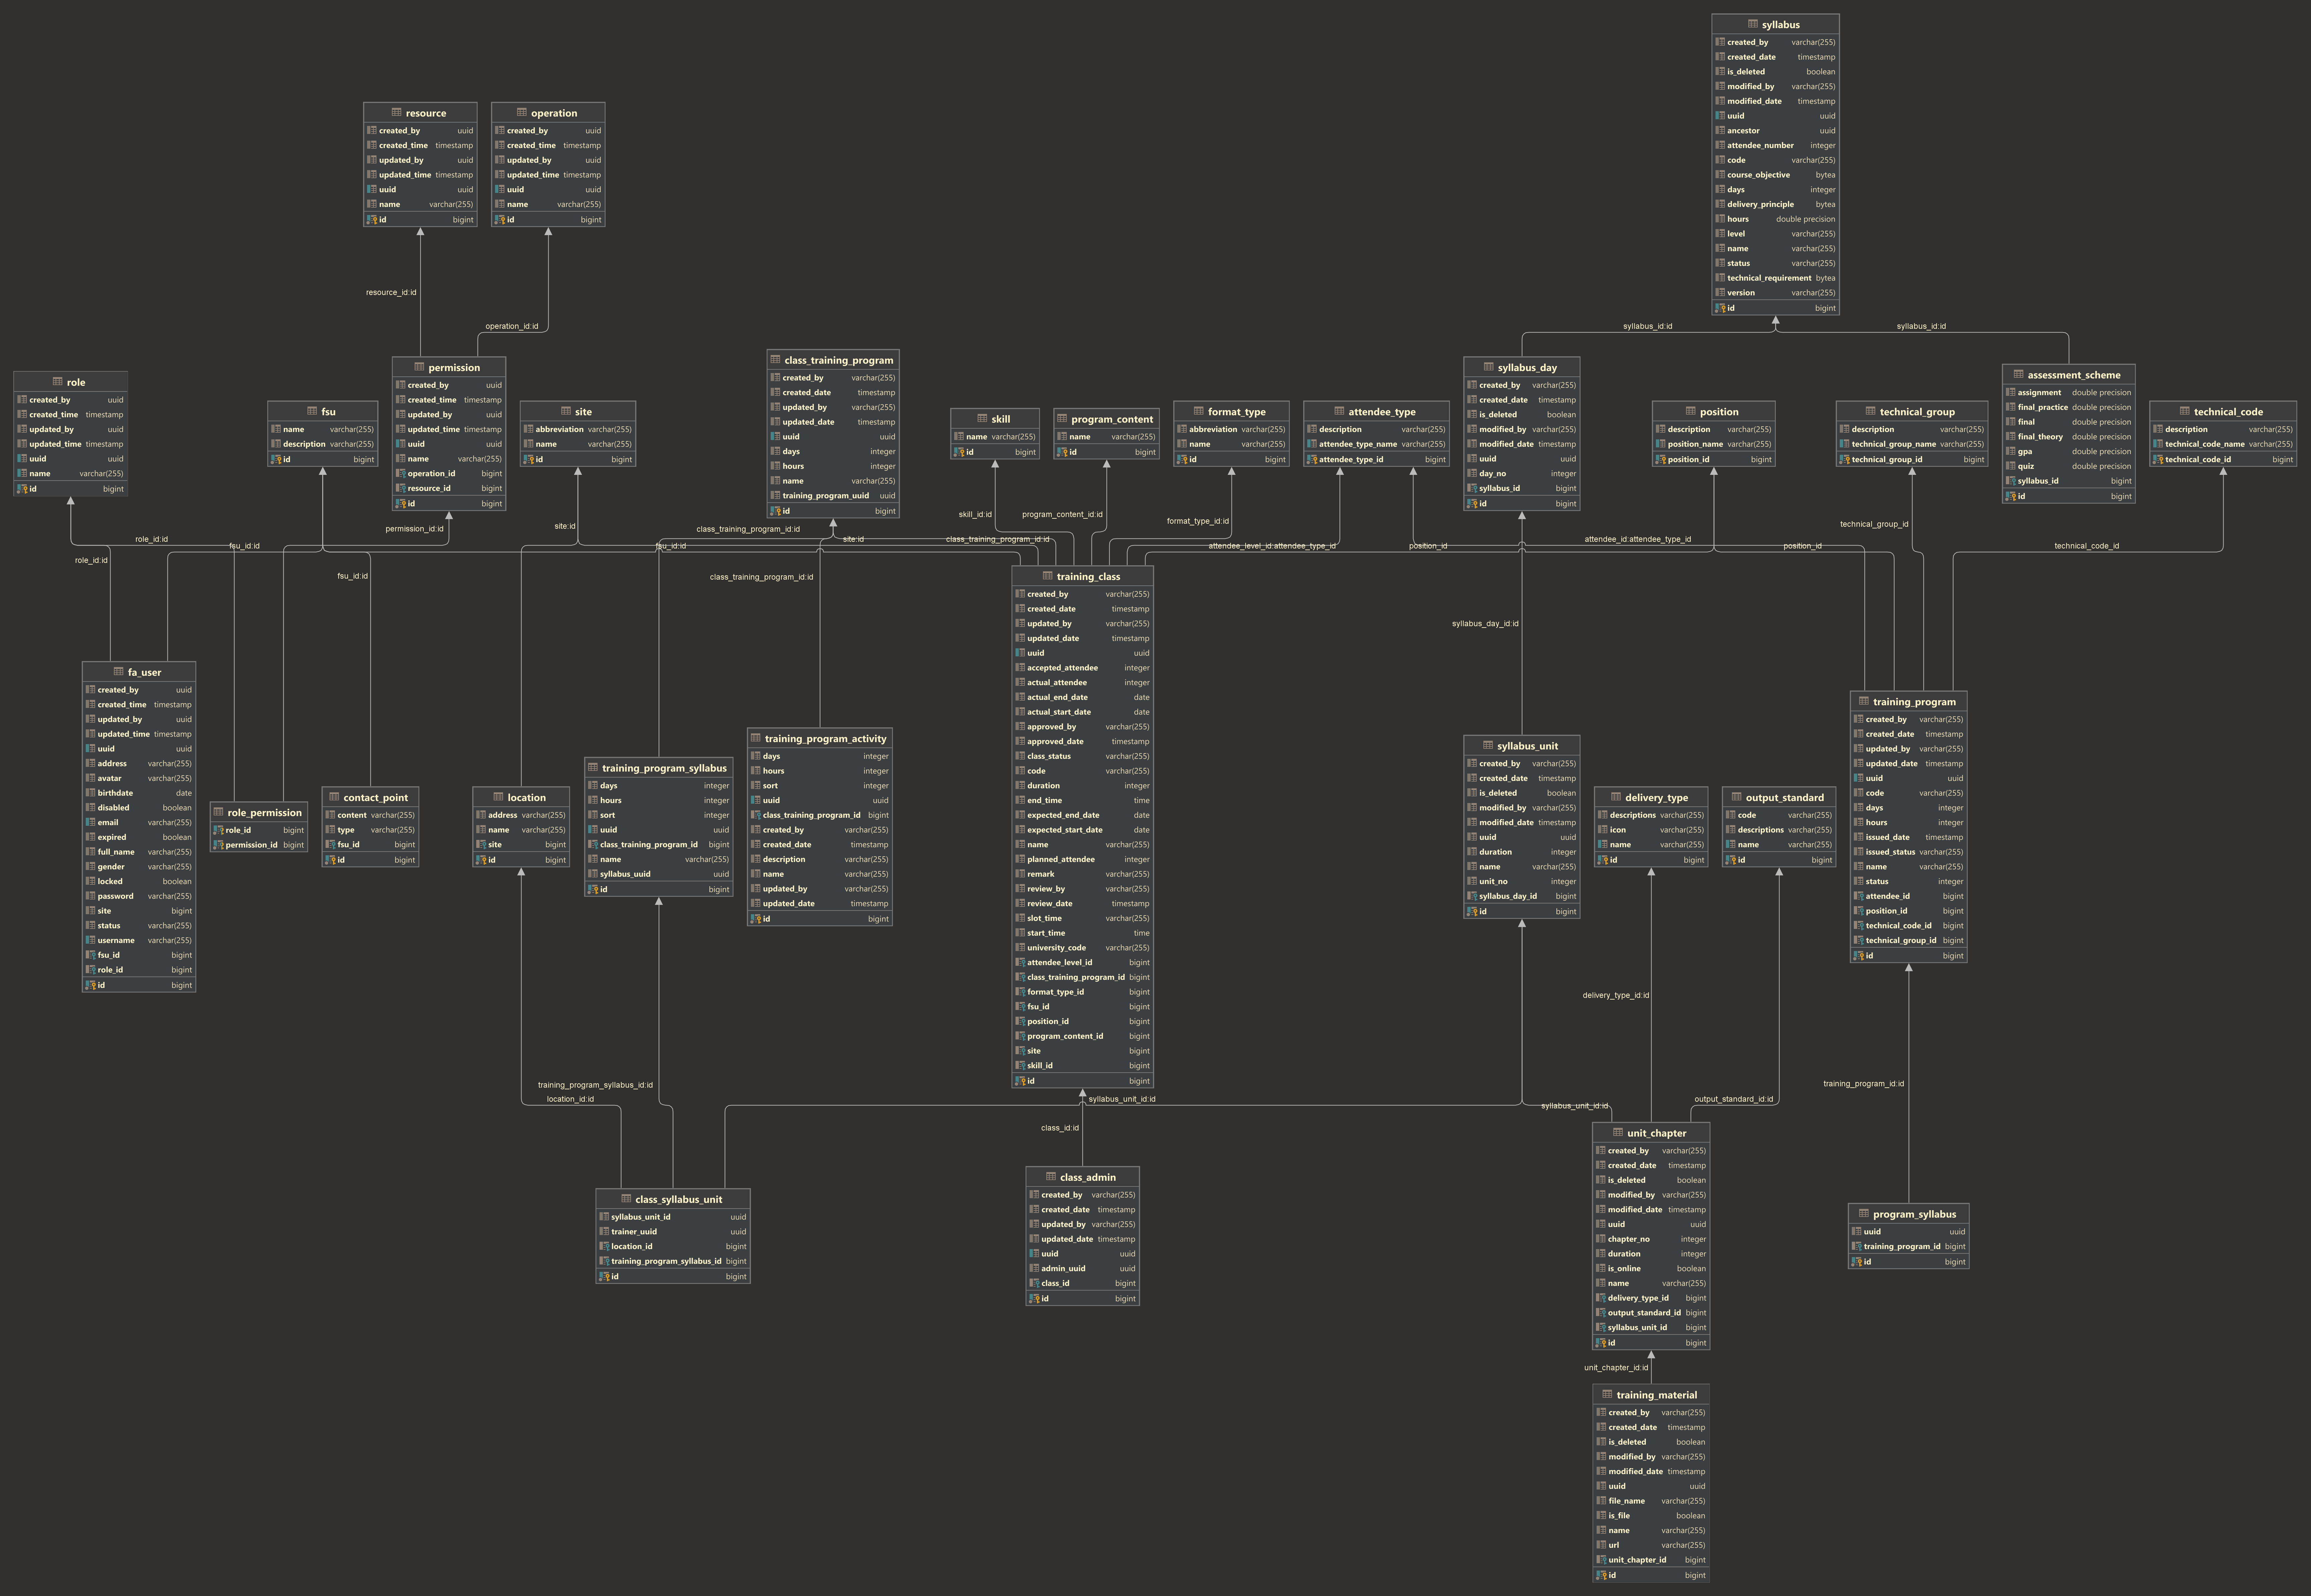
\includegraphics[width=500px]{../meta/db.diagrams.png}
\caption{Sơ đồ cơ sở dữ liệu}
\par
}
\end{figure}
\FloatBarrier

\end{document}
